% MSR 2027 Mining Challenge (SpecMine). Instruções em docs/OVERLEAF.md.
% Regras do site (https://2027.msrconf.org/track/msr-2027-mining-challenge, lidas em 07/nov/2026):
%   IEEE conference template, \documentclass[10pt,conference]{IEEEtran}; 4 páginas + 1 só de referências (estrito);
%   duplo-cego (sem nomes; trabalho próprio citado em 3ª pessoa); seção própria de ética; dizer a versão do SpecMine.
% Números: todos saem de scripts/reproduzir.sh (docs/key_numbers_final.json, data/derived/tables/,
% data/validation/resultado_p4.csv, que é a RQ2; os arquivos dela se chamam p4_*).
\documentclass[10pt,conference]{IEEEtran}
\usepackage{cite}
\usepackage{amsmath,amssymb,amsfonts}
\usepackage{graphicx}
\usepackage{booktabs}
\usepackage{textcomp}
\usepackage{xcolor}
\usepackage[hidelinks]{hyperref}
\usepackage{tikz}
\usetikzlibrary{arrows.meta,decorations.pathreplacing}
\graphicspath{{figs/}}

\begin{document}

\title{Editing and Spec Decay in Spec-Driven Development}

% Versão identificada; anonimizar novamente antes de uma submissão duplo-cega.
\author{\IEEEauthorblockN{João Pedro Laureano}}

\maketitle

\begin{abstract}
Spec-driven development (SDD) is an emerging practice in which natural-language specifications guide coding agents. Using SpecMine v1.0, we study how these specifications evolve after creation: how often they are revised, and how often code changes leave them outdated. We measure edit rates by tool and read 280 pairs of an OpenSpec living specification and a later pull request that changed linked code without updating it. Most specs had no later commit by July 11, 2026. OpenSpec living specs were edited more often than Spec Kit specs, although the difference was small. Of the 270 judgeable pairs, the mean per-repository share whose spec became false was 5.4\%; counting specs that also failed to describe new behavior within their scope raised it to 10.6\%. In 11 pairs, the changed behavior was outside the focal spec's scope, and our search found no other spec describing it. Treating these gaps as decay raised the estimate to 14.9\% (95\% CI 9.5--20.8).
\end{abstract}

\begin{IEEEkeywords}
spec-driven development, specifications, documentation decay, software evolution, mining software repositories
\end{IEEEkeywords}

\section{Introduction}
In spec-driven development (SDD), a natural-language specification guides a coding agent. After implementation, the spec can remain in the repository and guide later work. Agarwal et al.'s SpecMine corpus records these files and their commit histories~\cite{agarwal2026sdd}.

OpenSpec keeps each proposed change in a separate folder. Once the work is complete, \emph{archiving} merges its proposed spec edits into the capability's \emph{living spec} and moves the change folder to \texttt{changes/archive/}. The living spec remains in \texttt{openspec/specs/} for later work~\cite{openspecdocs}. In Spec Kit, a feature description becomes a spec in its own branch; an implementation plan and task list then guide coding~\cite{speckitdocs}. B\"ockeler classifies Spec Kit as \emph{spec-first}; by her definitions, OpenSpec is \emph{spec-anchored}, since its living specs are kept after the task~\cite{bockeler2025sdd}.

Because a living spec guides later work, code changes without a matching update may leave it describing obsolete behavior or omitting new behavior. An agent using it may carry those errors into the next task. SpecMine's interviews identified this risk as \emph{spec decay}, but the study did not measure how often it occurs. Our research question is: \textbf{How do SDD specifications evolve after creation, and do they stay accurate as the code changes?} We answer it through two subquestions:

\begin{itemize}
\item \textbf{RQ1:} How often are specs edited after creation, and does this differ between tools?
\item \textbf{RQ2:} When a pull request (PR) changes the code linked to a living spec but leaves the spec unchanged, how often does the spec become false or incomplete (spec decay)?
\end{itemize}

SDD assumes that a spec keeps guiding work after it is written, which holds only if specs are kept current; RQ1 tests whether they are, and whether tools differ. RQ2 then asks whether a living spec that is not updated still describes the system. We formulated the hypotheses after exploring the dataset, drawing on literature and tool documentation. We fixed the decision rules before the main labeling, but did not preregister them.

\section{Related Work}
Agarwal et al.\ introduced SpecMine and studied SDD through Reddit posts, 21 interviews, and 266 repositories. They found that 81.5\% of specs had one commit; 7 interviewees raised spec decay as a concern~\cite{agarwal2026sdd}. Claudino et al.'s EPIC offers 40 practices for writing SDD artifacts, derived from 114 repositories; it assesses artifact quality at one point, leaving accuracy after code changes open~\cite{claudino2026epic}. For documentation, Aghajani et al.\ define an outdated document as one ``not in sync with other parts of a system'' whose information ``was correct and complete before a change was introduced''~\cite{aghajani2019issues}. Tan et al.\ found that most of the more than 3,000 GitHub projects they studied at some point had documentation referring to code elements that had been deleted~\cite{tan2024outdated}. Agarwal et al.\ call a spec left false or incomplete by later code changes \emph{spec decay}; \emph{implementation drift} describes an agent departing from the spec during implementation~\cite{agarwal2026sdd}.

\section{Study Design}
\subsection{Data and Units}
We use SpecMine v1.0 (July 2026 snapshot)~\cite{specmine2026}: 470,795 spec files in 73,031 repositories (73,030 in~\cite{agarwal2026sdd}), with the commit history of each file path. SpecMine fetched commit histories on July 11, 2026, and spec contents on July 12; we ignore commits and PRs dated after July 11 (UTC) and use each spec's text as fetched (none of the 280 RQ2 specs changed between the two dates). SpecMine collected PRs only from repositories with at least 10 stars~\cite{agarwal2026sdd}. We exclude 14,262 \texttt{caffeine.ai} specs across 13,749 repositories: the service creates one repository per generated app~\cite{agarwal2026sdd}, so including them would give one generator disproportionate weight in our repository-level estimates. For life-cycle analyses, we also remove files with no commit history in SpecMine (1,473), since their edits cannot be counted; files whose content appears in at least five repositories; and repositories where at least half the specs have such copied content. These copies include templates and tutorials, which would inflate the share of specs with no recorded later edit. The resulting corpus has 447,795 specs in 57,435 repositories. Groups are OpenSpec, Spec Kit, other named tools, and specs without a tool (generic paths such as \texttt{specs/}). Unless stated otherwise, estimates are means of per-repository proportions, so that large repositories do not dominate, with 95\% confidence intervals from 1,000 bootstrap resamples of repositories. A threshold criterion is \emph{met} when the whole interval lies on the predicted side, \emph{refuted} when it lies on the other side, and \emph{inconclusive} otherwise.

\subsection{RQ1: Editing}
RQ1 marks each spec as \emph{edited} if its path has a second commit by July 11, regardless of age, and reports the share of edited specs in each group. \textbf{H1:} OpenSpec living specs are edited more often than Spec Kit specs. Living specs are spec-anchored and meant to be maintained, while Spec Kit specs are spec-first~\cite{bockeler2025sdd}, so we expect more edits to living specs. H1 requires both nonoverlapping 95\% intervals and a significant one-sided Mann--Whitney test on the per-repository proportions; Cliff's $\delta$ gives the effect size. Spec Kit specs are older (median 101 days versus 69 for living specs), giving them more time to be edited. As a sensitivity check, we use a common 60-day window, shorter than both median ages: among specs at least 60 days old on July 11, we record whether a second commit occurred within 60 days of creation.

\subsection{RQ2: Spec Decay}
\subsubsection{Pair selection}
OpenSpec keeps a living spec for each capability. We link it to code files named in the \texttt{tasks.md} files of changes to that capability. To limit ambiguous links to files that may serve several capabilities, we require a directory in the cited path and exclude generic basenames such as \texttt{index} and \texttt{utils}.\footnote{Excluded basenames, with any extension: \texttt{index}, \texttt{main}, \texttt{app}, \texttt{util(s)}, \texttt{helper(s)}, \texttt{type(s)}, \texttt{constant(s)}, \texttt{config}.} A candidate pair (Fig.~\ref{fig:pair}) is one living spec and one PR merged after its last edit but by July 11. The PR must modify linked code without touching a spec for that capability. Several linked files in one PR still form one pair. With no spec edit between the PR and July 11, the fetched text is also the text at PR merge; two timestamp exceptions appear in Section~\ref{sec:threats}.

The 108 eligible repositories contained 13,028 candidate pairs. We sampled up to three spec--PR pairs per repository (289 selected). We fixed that cap before full labeling: assuming a 12.5\% decay rate, from a preliminary large language model (LLM) labeling of the pilot pairs (the pairs labeled first), and within-repository correlation $\rho \le 0.3$, the upper confidence limit fell below our 20\% cutoff in at least 80\% of simulated samples. The GitHub API returned diffs for 280 pairs; one author read all 280, and 270 were judgeable (198 distinct PRs, 239 specs).

\begin{figure}[t]
\centering
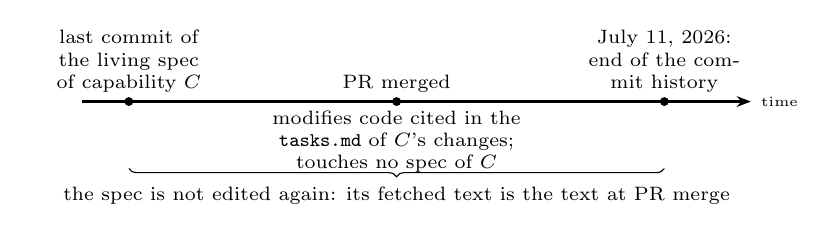
\begin{tikzpicture}[font=\scriptsize, ev/.style={align=center, text width=25mm, inner sep=1pt}]
\draw[-{Stealth[length=1.8mm]}, thick] (0,0) -- (8.5,0) node[right, font=\tiny]{time};
\foreach \x in {0.6,4.0,7.4} \fill (\x,0) circle (1.6pt);
\node[ev, above] at (0.6,0.08) {last commit of the living spec of capability $C$};
\node[ev, above] at (4.0,0.08) {PR merged};
\node[ev, below, text width=36mm] at (4.0,-0.08) {modifies code cited in the \texttt{tasks.md} of $C$'s changes; touches no spec of $C$};
\node[ev, above] at (7.4,0.08) {July 11, 2026: end of the commit history};
\draw[decorate, decoration={brace, amplitude=3pt, mirror}] (0.6,-0.85) -- (7.4,-0.85) node[midway, below=3pt, font=\scriptsize]{the spec is not edited again: its fetched text is the text at PR merge};
\end{tikzpicture}
\caption{One RQ2 pair on a timeline. A human reads the spec and the diff of the linked code to judge decay.}
\label{fig:pair}
\end{figure}

\subsubsection{Labeling codebook}
For each pair, the rater read the full spec and the diff of the linked files and answered, in order: (1) does the diff change observable behavior? If not, \emph{preserves}; (2) is that behavior within this spec's subject? If not, \emph{other capability}; (3) does a sentence of the spec become false? If so, \emph{contradicts}; otherwise, if the spec does not cover the new behavior within its scope, \emph{omits}; missing information yields \emph{cannot judge}. Pairs in which the code already contradicted the spec before the PR are excluded (3 pairs; \emph{prior divergence} in Fig.~\ref{fig:flow}).

\subsubsection{Owner check}
\emph{Other capability} is accepted only if another spec in the repository describes the changed behavior or, more loosely, the component it changes (9 pairs; a sensitivity row of Table~\ref{tab:decay} counts them as decay). An LLM reviewer (Claude), blind to the second rater's labels, searched candidates (specs whose \texttt{tasks.md} cites the same file, specs touched by the PR, specs sharing rare identifiers with the diff); without evidence the pair counts as \emph{omits}, unless the human rater vetoed it, confirming that the behavior is outside the spec's scope although the search found no spec describing it. Of 128 such labels, 115 were confirmed, 13 lacked evidence, and the rater vetoed 12. After quoting the scope passage behind each veto, the rater withdrew one (it counts as \emph{omits}).

\subsubsection{Second rater and adjudication}
For an independent comparison, DeepSeek v4 Pro applied the same codebook to all 280 pairs without seeing the human labels. As fixed before labeling, agreement is measured on the 222 pairs outside the pilot. On the 28 pairs where the human and the LLM disagreed on decay (yes/no), the human re-read the pair seeing both readings, unattributed and in random order, and set the final label. Every final pair label is a human judgment.

\subsubsection{Measures}
$Y$ is the share of judgeable pairs whose spec \emph{contradicts} or \emph{omits} (broad, our criterion, matching the definition of decay) or only \emph{contradicts} (strict), computed per repository and averaged. \textbf{H2:} a relevant share of these PRs leaves the spec out of date. In SpecMine's study, 7 interviewees raised spec decay as a concern~\cite{agarwal2026sdd}, and outdated documentation is a known problem~\cite{aghajani2019issues,tan2024outdated}; if decay were frequent, living specs would mislead later work. We chose interpretive bands before labeling: an interval entirely below 20\% is a \emph{negative result}; within 20--50\%, co-change with some decay; at least 50\%, decay. These cutoffs express how frequent decay must be to change our conclusion, rather than rates established by prior work. We also report $X$, the share of linked living specs that experienced at least one such PR.

\section{Results}
\begin{table}[t]
\centering
\caption{RQ1 by tool: \% of specs edited after creation (per repository, 95\% CI) and, among specs at least 60 days old, \% edited within their first 60 days.}
\label{tab:rq1}
\footnotesize
\begin{tabular}{@{}lcc@{}}
\toprule
Group & Edited & Within 60 days \\
\midrule
OpenSpec living & 28.4 [27.5, 29.2] & 28.9 \\
Spec Kit & 22.9 [22.2, 23.5] & 22.7 \\
Other tools & 17.8 [16.5, 19.1] & 17.2 \\
No tool & 40.0 [39.6, 40.5] & 38.1 \\
\bottomrule
\end{tabular}
\end{table}

\begin{figure*}[t]
\centering
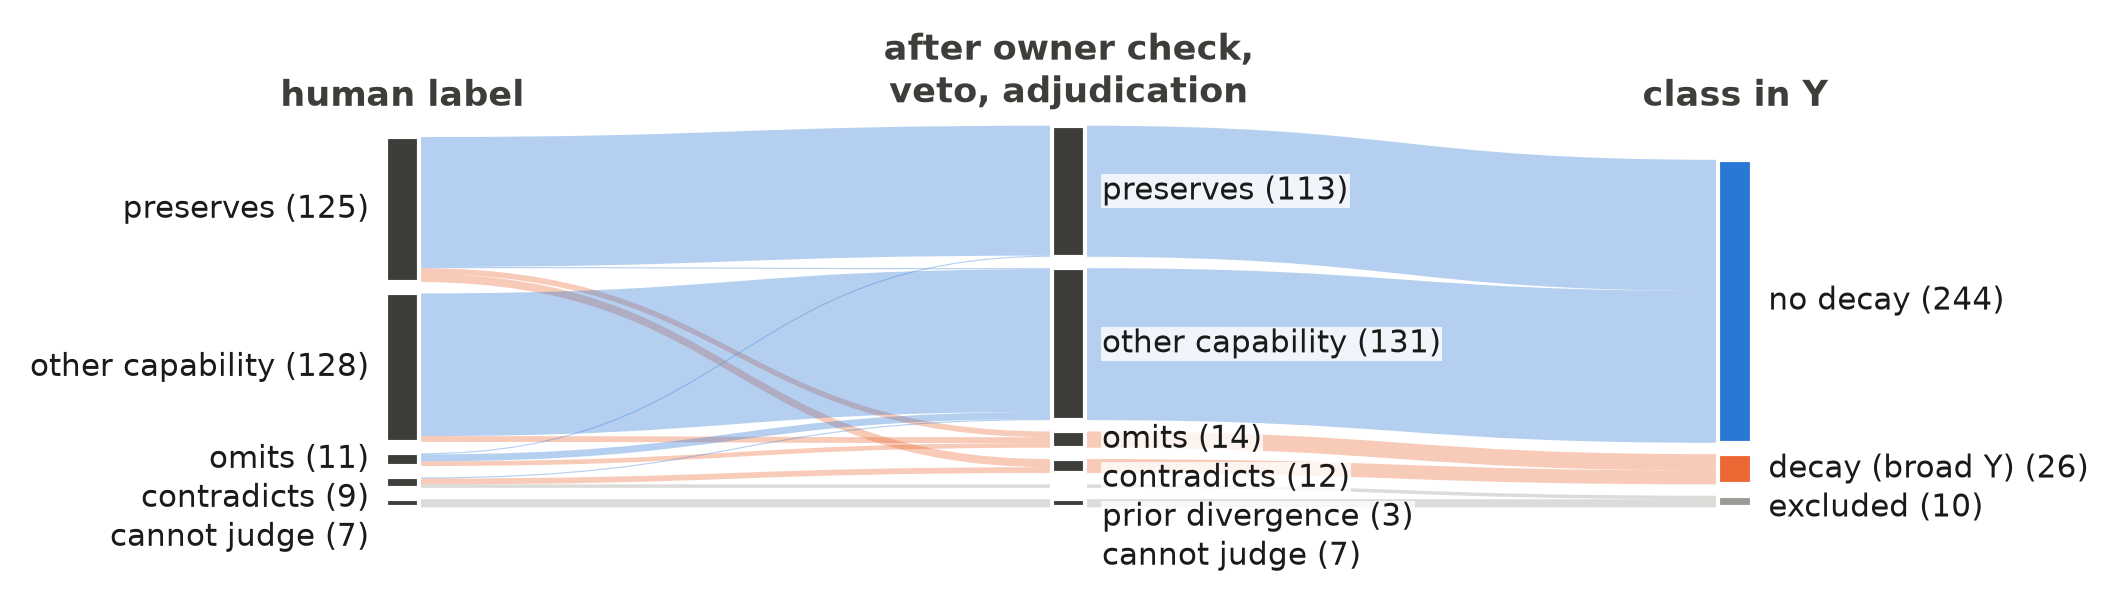
\includegraphics[width=\textwidth]{p4_flow}
\caption{RQ2 labels from the human rater to the class used in $Y$ (counts of pairs; $Y$ itself is a mean per repository). Blue: no decay; orange: decay; gray: excluded.}
\label{fig:flow}
\end{figure*}

\subsection{RQ1: Most Specs Have One Recorded Commit}
By July 11, fewer than half of the specs in each group had been edited (Table~\ref{tab:rq1}). OpenSpec living specs were edited 5.5 percentage points more often than Spec Kit specs; their intervals are disjoint and $p < 0.001$, but Cliff's $\delta = 0.17$ indicates a small effect (H1 met). The order also holds in the fixed 60-day window (28.9\% vs.\ 22.7\%).

\subsection{RQ2: Living Specs Rarely Become False}
\begin{table}[t]
\centering
\caption{RQ2: spec decay $Y$ (\% of judgeable pairs, mean per repository, 95\% CI). Main: owner check, veto, and adjudication. Strict $Y$ stays below 20\% everywhere; broad $Y$ crosses it when specification gaps count as decay and, by 0.1 points, for older PRs.}
\label{tab:decay}
\footnotesize
\setlength{\tabcolsep}{3pt}
\begin{tabular}{@{}lccc@{}}
\toprule
Analysis & Pairs & Broad $Y$ & Strict $Y$ \\
\midrule
\textbf{Main} & 270 & \textbf{10.6} [5.9, 16.0] & 5.4 [2.2, 9.5] \\
Excluding pilot pairs & 213 & 10.2 [5.7, 15.2] & 4.4 [1.5, 7.9] \\
Before adjudication & 270 & 7.3 [4.1, 10.8] & 2.7 [0.8, 5.2] \\
Component-level owner = decay & 270 & 13.5 [8.7, 18.9] & 5.4 [2.2, 9.5] \\
\textbf{Spec. gaps = decay} & 270 & 14.9 [9.5, \textbf{20.8}] & 5.4 [2.2, 9.5] \\
Gaps and component = decay & 270 & 17.8 [12.4, \textbf{24.0}] & 5.4 [2.2, 9.5] \\
\emph{Cannot judge} = decay & 277 & 12.4 [7.6, 18.1] & 7.3 [3.5, 11.7] \\
PRs $\ge$60 days old & 119 & 12.3 [4.7, \textbf{20.1}] & 6.3 [0.0, 13.2] \\
\bottomrule
\end{tabular}
\end{table}

Such PRs are common: $X = 28.3\%$ [24.0, 32.7] of linked living specs (in the 190 repositories with PR data) had at least one PR that changed their code without touching any spec of their capability. In the 280 pairs, the human labels were 125 \emph{preserves}, 128 \emph{other capability}, 11 \emph{omits}, 9 \emph{contradicts}, and 7 \emph{cannot judge}. After the owner check, the veto, and adjudication (Fig.~\ref{fig:flow}), the spec became false in 5.4\% [2.2, 9.5] of the pairs (strict $Y$, mean per repository; 12 of 270 pooled), a negative result in every analysis of Table~\ref{tab:decay}. It became false or incomplete in $Y = 10.6\%$ [5.9, 16.0] (broad $Y$; 26 of 270 pooled), also a negative result under the main rule (H2 refuted), including without the pilot pairs. As a sensitivity check, we restrict RQ2 to 119 pairs with no spec update for at least 60 days between PR merge and July 11; $Y = 12.3\%$ [4.7, 20.1], inconclusive by 0.1 points. In 11 pairs, the rater placed the changed behavior outside the spec's scope, and the reviewer found no other spec describing it; absence remains unproven. We named these \emph{specification gaps} after seeing the data. Our pre-declared rule gave the rater a veto, but we made the vetoed reading the main analysis only after seeing the labels; the rater kept the veto on all 11 pairs. Counting these gaps as decay instead raises $Y$ from 10.6\% to 14.9\% [9.5, 20.8], making H2 inconclusive under our bands.

In 131 of the 280 pairs the label ends as \emph{other capability}. In 111 of them another spec of the repository describes the changed behavior, in 9 another spec covers only the component, and 11 are the specification gaps discussed above. Decay concentrates in some repositories: the observed intra-repository correlation (0.32 broad, 0.43 strict) exceeds the $\rho \le 0.3$ assumed when sizing the sample; since the interval already excludes the threshold, the verdict is unaffected.

Agreement between the human rater and DeepSeek outside the pilot was weak: $\kappa = 0.33$ over the five labels (222 pairs) and $0.23$ for decay yes/no (213 judgeable pairs), although the two labeled a similar number of pairs as decay (17 by the human and 23 by the LLM, of 213). The disagreements that affect $Y$ follow two opposite patterns. In 13 pairs the human saw no behavior change (\emph{preserves}) where the LLM labeled \emph{omits} or \emph{contradicts}, typically for new details the spec does not mention (a new CLI flag or health probe); the human judged the spec still true at its own level of abstraction. In 7 pairs the human labeled \emph{omits} where the LLM found another spec owning the behavior. Adjudication moved 15 pairs into decay and 8 out.

\section{Discussion}
\emph{Feared, but rare.} Practitioners told Agarwal et al.\ that specs go stale as code changes~\cite{agarwal2026sdd}, and studies of conventional documentation report outdated content~\cite{aghajani2019issues,tan2024outdated}. Yet in our pairs, a PR that changed linked code rarely left an OpenSpec living spec false. The units differ, so we compare directions, not rates. Our data fit three explanations. OpenSpec updates the living spec when a change is archived~\cite{openspecdocs}, so behavior specified through the workflow reaches it; the behavior a PR changes may belong to another spec; and a spec written at the level of intent is untouched by code changes below that level.

\emph{Decay crosses capabilities.} Agarwal et al.\ report that ``Spec decay affects living specs, mainly when changes alter behavior that other specs describe''~\cite{agarwal2026sdd}. Our candidate pairs have this shape by construction: SpecMine records PRs that touch some spec, so nearly every candidate PR updated a spec other than the focal one. In 111 sampled pairs, another spec, as fetched, describes the changed behavior; we cannot date that description to the PR, so the change may have reached a spec, just not the focal one. The 11 gaps with no known owner decide whether broad decay falls below 20\%.

\emph{How detailed must a spec be?} Our codebook does not fix the required detail. Where the human and the LLM disagreed on decay, a recurring case was a new detail, such as a CLI flag, that the spec does not mention: the LLM read an omission, the human a change below the spec's level of abstraction. This is the measurement side of Agarwal et al.'s observation that ``a spec that specifies more implementation detail decays sooner''~\cite{agarwal2026sdd}: the more detail a spec is expected to hold, the more changes count as decay. EPIC assesses how SDD artifacts are written~\cite{claudino2026epic}; a practice stating the level of detail a spec commits to would make omissions decidable.

\emph{Spec-anchored in practice.} RQ1 supports B\"ockeler's distinction~\cite{bockeler2025sdd}: living specs, meant to be maintained, are edited more often than spec-first Spec Kit specs. A living spec that is not edited is not necessarily stale: RQ2 shows that, after linked code changes, it rarely becomes false.

\emph{LLMs as second raters.} Agreement between the human and DeepSeek was weak, so we used the LLM as a check, not a substitute, in line with Ahmed et al., who conclude that current models cannot replace all human annotators~\cite{ahmed2025llm}. As a check it was useful: adjudication moved pairs in both directions and raised $Y$.

\emph{Implications.} For tools, the specification gaps point to behavior that no capability owns, so coverage across capabilities may matter as much as keeping each spec in sync. For research, commit counts cannot show decay~\cite{agarwal2026sdd}; measuring it requires reading the spec against the change.

\section{Threats to Validity}\label{sec:threats}
\emph{Construct.} RQ1 tracks current paths, so it misses history across renames; squashed or rebased commits also ``merge several edits into one''~\cite{agarwal2026sdd}, which may undercount edits made on feature branches, as in Spec Kit. SpecMine's data confirm the \texttt{tasks.md} link in 279 of 280 pairs but cannot establish behavior ownership or the commit used to resolve a path. \emph{Omits} depends on expected spec detail (Discussion).

\emph{Internal.} RQ2 rests on one human rater, who also adjudicated the disagreements with the LLM, which is weaker than an independent second human. The owner check was performed by an LLM reviewer with human veto; its recall is unknown, and removing it lowers broad $Y$ to 6.7\%. The 11 specification gaps rest on the rater's scope judgment, without a documentary owner. The category was named, the vetoed reading was made the main analysis, and the scope passages were quoted after the results were known; the withdrawn veto raised $Y$. In 2 of the 280 pairs the spec's last commit was authored before but committed after the PR merge, so the fetched text might postdate the PR; one of them counts as decay.

\emph{External.} SpecMine covers public GitHub spec files first committed in 2024--2026, mostly in young repositories; 98.3\% of spec files with a recorded history have a single author~\cite{agarwal2026sdd}. RQ2 is restricted to OpenSpec living specs in repositories with at least 10 stars and to PRs that touch some spec: PRs that change code without touching any spec are outside the data, so our result does not cover decay outside the SDD workflow. Specs abandoned and deleted are invisible (survivorship). Updates after July 11 are unobserved.

\emph{Conclusion.} RQ2 is relational, not causal. Sensitivity analyses not shown in Table~\ref{tab:decay} are in the replication package. The order of decisions is recorded in dated documents, not in an external preregistration.

\section{Ethical Considerations}
We use public data under the GitHub API terms; our collections removed e-mails, commit signatures, and avatars, never stored access tokens, and we report only aggregates. \emph{Use of AI.} Following Wagner et al.~\cite{wagner2025guidelines}, we document LLM use. DeepSeek v4 Pro (temperature 0.3, November 2026) was the second rater for RQ2; Claude Opus 5.5 reviewed the owner evidence (human veto) and assisted with programming and with drafting this text. LLMs also translated Chinese-language specs for reading, produced the preliminary pilot labels used only to size the RQ2 sample, and critiqued the study design; every final label is a human decision. The DeepSeek prompts, the owner-check criterion, model versions, and dates are in the replication package. The authors verified all content and are responsible for it.

\section{Data Availability}
The replication package\footnote{\url{https://github.com/joaolaureano/spec-lifecycle-replication}} contains all scripts, the frozen API collections with checksums, every label and decision, and a script that runs the full pipeline twice and checks that all outputs are identical.

\section{Conclusion}
Most specs had no later commit by July 11, 2026, and OpenSpec living specs were edited more often than Spec Kit specs, by a small margin. Among PRs touching some spec, linked code changes left the focal living spec false in 5.4\% of pairs and false or incomplete in 10.6\% (repository means), both with intervals below 20\%. The latter becomes inconclusive for pairs with no spec update for 60 days or when 11 specification gaps count as decay. An open question is which spec should own behavior that none describes.

\bibliographystyle{IEEEtran}
\bibliography{refs}

\end{document}
